\section{Theorie}
\label{sec:Theorie}
Die Stabilität eines Atomkerns wird maßgeblich durch das Zahlenverhältnis von Neutronen zu Protonen bestimmt. Liegt die Neutronenzahl etwa um $\SI{20}{\percent}$ bis $\SI{50}{\percent}$ über der Protonenanzahl, ist der Kern stabil.

Als Maß für die Zerfallswahrscheinlichkeit wird die Halbwertszeit bezeichnet. Diese ist definiert als die Zeit, nach der genau die Hälfte der Menge der ursprünglich vorhandenen Kerne zerfallen ist.
Im vorliegenden Versuch werden sinnigerweise Isotope untersucht, deren Halbwertszeit im Rahmen von wenigen Minuten bis Stunden liegt.
So geartete Isotope müssen zunächt allerdings erzeugt werden. Dazu werden zunächst stabile Atomkerne mit Neutronen beschossen. Die erzeugten Isotope sind recht instabil, sodass ihre Halbwertszeit im geforderten Rahmen liegt.


\subsection{Aktivierung mit Neutronen}
Wechselwirkungen zwischen Teilchen und Kernen werden als Kernreaktionen bezeichnet.
Die ablaufende Reaktion bei Beschuss eines Kerns $A$ mit einem Neutron lässt sich wie folgt schreiben:
\begin{align}
  \ce{^{m}_{z}A+ ^{1}_0n -> ^{m+1}_zA^{*} -> ^{m+1}_zA +\gamma}
\end{align}
Wird ein Kern $A$ mit einem Neutron beschossen, wird zunächst ein sogenannter \textbf{Zwischenkern} $\ce{A^{*}}$, auch \textbf{Coupondkern} genannt, erzeugt. Die zusätzlich eingebrachte Energie gegenüber dem Kern $A$ durch die kinetische Energie und die Bindungsenergie des Neutrons wird auf eine große Anzahl an Nukleonen im Kern verteilt.
Nach einer kurzen Zeitspanne von $\SI{10e-16}{\second}$ geht der Zwischenkern unter Emission eines $\gamma$-Quants in seinen Grundzustand zurück.
Der so erzeugte Kern $\ce{^{m+1}_zA }$ hat allerdings ein Neutron zuviel, sodass er instabil ist.
Unter Emmission eines Elektron geht dieser wieder in einen stabilen Zustand über:
\begin{align*}
\ce{^{m+1}_zA -> ^{m+1}_{z+1}C +\beta ^{-} + E_{\mathrm{kin }}+ \bar{\symup{\nu}}_e}
\end{align*}

In der Kernphysik ist der Wirkungsquerscchnitt $\sigma$ ein Maß dafür, mit welcher Wahrscheinlichkeit ein Neutron durch einen stabilen Kern eingefangen wird.
Nach Breit und Wigner lässt sich der Wirkungsquerschnitt als Funktion der Neutronenenergie $E$ darstellen:
\begin{equation}
  \sigma (E)=\sigma _0 \sqrt{\frac{E_{\mathrm{r}_i}}{E}}\frac{\tilde{c}}{\left(E-E_{\mathrm{r}_i}\right)^2 +\tilde{c}} \text{.}
\end{equation}
Hierbei stellt $E_{\mathrm{r}_i}$ die Energieniveaus des Zwischenkerns $A^{*}$ dar und $\tilde{c}$ sowie $\sigma_0$ sind für die betreffende Kernreaktion charakteristische Konstanten.
Ist die Summe $E$ aus der kinetischen Energie und der Bindungsenergie des einfallenden Neutrons sehr viel kleiner als die Energieniveaus des Zwischenkerns $E_{\mathrm{r}_i}$, so wird der Nenner des Bruchs im Wirkungsquerschnitt praktisch konstant. Da die Energie $E$ des einfallenden Neutron proportional zu $v^2$ ist, ergibt sich somit:
\begin{equation}
  \label{eqn:siggi}
  \sigma \propto \frac{1}{\sqrt{E}}\propto \frac{1}{v} \text{.}
\end{equation}

\subsection{Erzeugung niederenergetischer Neutronen}
Nach der Überlegung \ref{eqn:siggi} ergibt sich besonders für niederenergetische Neutronen also eine hohe Wahrscheinlichkeit für Kernreaktionen.
Neutronen sind instabil und müssen daher zunächst über geeignete Kernreaktionen erzeugt werden.
Im vorliegenden Versuch werden hierzu $\ce{^{9}Be}$-Kerne mit $\alpha$-Teilchen beschossen und hierbei Neutronen freigesetzt:
\begin{align}
    \ce{ ^{9}_4Be + ^{4}_2He^{2+}  -> ^{12}_6C + ^{1}_0n}\text{.}
\end{align}
Um die kinetische Energie und damit die Geschwindigkeit der $\alpha$-Teilchen zu verringern, diffundieren die Neutronen nach dem Austritt aus der Neutronenquelle zunächst durch eine Mantelschicht aus Paraffin. Im Paraffin finden elastische Stöße zwischen den Neutronen und dem Paraffin statt. Durch die elastischen Stöße wird das Neutron recht effektiv gebremst, da die Stoßpartner annähernd gleich groß sind.
Die Neutronen werden gebremst bis auf eine Energie von etwa $\SI{0.025}{\electronvolt}$ bei $T=\SI{290}{\kelvin}$. Sie haben hierbei eine mittlere Geschwindigkeit von $\bar{v}=\SI{2.2}{\kilo\meter\per\second}$. Neutronen mit den genannten Eigenschaften werden als \textbf{therminsche Neutronen} bezeichnen.

\subsection{Untersuchung des Zerfalls instabiler Isotope}
Im vorliegenden Versuch wird zum einen Indium $\ce{^{115}_49In}$ mit einem einfachen Zerfall und Silber mit zwei parallel ablaufenden Zerfällen untersucht.
Für den Zerfall des Indium nach Beschuss mit Neutronen gilt:
\begin{align}
  \label{eqn:indium}
  \ce{^{115}_49In + n -> ^{116}_49In -> ^{116}_50Sn + \beta ^{-} + \bar{\symup{\nu}}_e} \text{ .}
\end{align}
Der Zerfall bei Silber stellt sich etwas komplizierter dar.
Natürliches Silber besteht nach \cite{silber} zu $\SI{51.8}{\percent}$ aus dem Isotop $\ce{^{107}Ag}$ und zu $\SI{48.2}{\percent}$ aus $\ce{^{109}Ag}$.
Es gelten die Reaktionsgleichungen:
\begin{gather}
  \label{eqn:silver}
  \ce{^{107}_47Ag + n -> ^{108}_47Ag -> ^{108}_48Cd + \beta^{-} + \bar{\symup{\nu}}_e}\text{ ,}\\
  \ce{^{109}_47Ag + n -> ^{110}_47Ag -> ^{110}_48Cd + \beta^{-} + \bar{\symup{\nu}}_e} \text{ .}
\end{gather}
Wird ein Silberblech mittels Neutronenbeschuss aktiviert, so laufen beide Zerfallsprozesse parallel ab. Es ist trotzdem eine Untersuchung der beiden einzelnen Zerfallsprozesse möglich, da die beiden Isotope mit hinreichend verschiedener Halbwertszeit zerfallen.
Nach hinreichend großer Zeitdauer ist das kurzlebige Isotop $\ce{^{110}Ag}$ und das langlebige Isotop $\ce{^{108}Ag}$ lässt sich nahezu isoliert beobachten.

Für radioaktive Zerfälle gilt das Zerfallsgesetz:
\begin{equation}
  \label{eqn:halbwertszeit}
  N(t)=N_0 \cdot \exp{(-\lambda t)} \text{.}
\end{equation}
Es ist $\lambda$ die materialspezifische Zerfallskonstante und $N_0$ die Anzahl der Kerne zu Beginn der Beobachtung.
Nach der Definition der Halbwertszeit ergibt sich diese zu:
\begin{gather*}
  \frac{1}{2} N_0= N_0 \cdot \exp{(-\lambda t)}\\
  \rightarrow T_{\frac{1}{2}}=\frac{\ln{2}}{\lambda} \text{ .}
\end{gather*}
Die Bestimmung der Halbwertszeit und der Zerfallskonstante über eine Messung der Zeitabhängigkeit der Kernanzahl $N(t)$ stellt sich als schwierig heraus.
Es wird daher die Anzahl $N_{\Delta t}(t)$ an Kernzerfällen in einem festen Zeitintervall $\Delta t$ bestimmt.
Mit der Definition
\begin{equation*}
  N_{\Delta t}(t)=N(t)-N(t+\Delta t)
\end{equation*}
ergibt sich für $N_{\Delta t}(t)$ nach Gleichung \eqref{eqn:halbwertszeit}:
\begin{equation}
  \label{eqn:Delta_t}
  N_{\Delta t}(t)=N_0 \cdot \exp{(-\lambda t)}-N_0 \cdot \exp{(-\lambda(t+\Delta t))} \text{.}
\end{equation}
Wird Gleichung \eqref{eqn:Delta_t} beidseitig logarithmiert, zeigt sich ein linearer Zusammenhang
\begin{equation}
  \label{eqn:ausgleichsrechnung}
  \ln{  N_{\Delta t}(t)}=\ln{N_0 \left(1- \exp{(-\lambda \Delta t}\right))}-\lambda t \text{ .}
\end{equation}
Hierbei ist die Wahl eines geeigneten Messintervalls $\Delta t$ nicht trivial und erfordert langwierige Vorversuche. Eine Liste mit geeeigneten Messintervallen liegt daher dem Experiment bei.
\begin{figure}
  \centering
  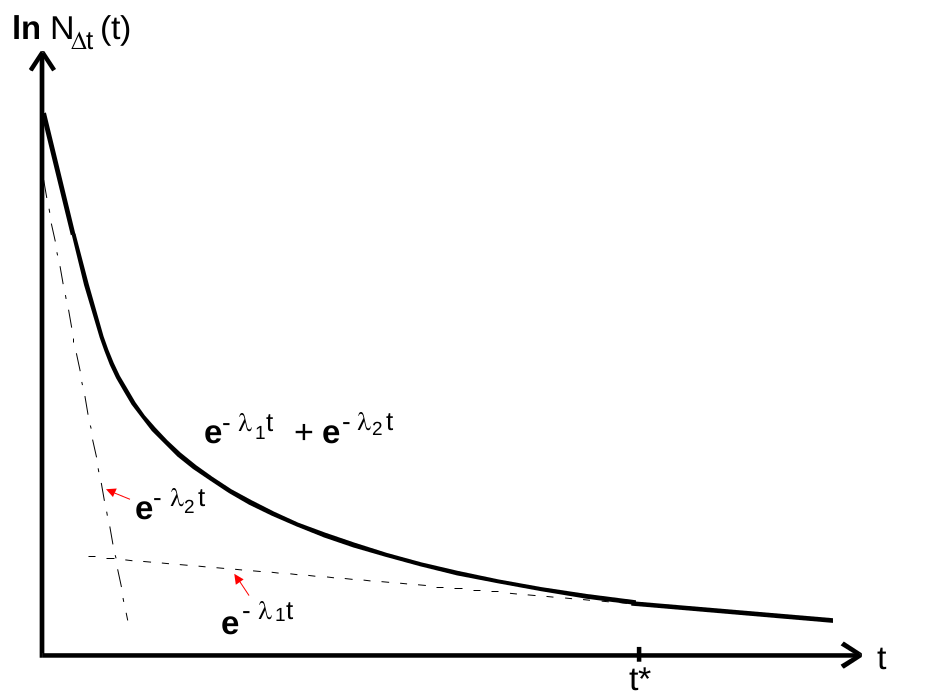
\includegraphics[width=0.7\textwidth]{Bilder/zerfallskurve.png}
  \caption{Prinzipielle Zerfallskurve eines Materials, welches aus zwei Isotopen mit sehr unterschiedlichen Zerfallskonstanten besteht.}
  \label{fig:zerfallskurve}
\end{figure}
Die verschiedenen Zerfälle beim Silber lassen sich wie folgt getrennt untersuchen:
Im Zerfalls-Diagramm (vgl. Abbildung \ref{fig:zerfallskurve}) ist ein Zeitpunkt $t^{*}$ so zu wählen, dass für alle $t_i>t^{*}$ die Zerfallskurve praktisch eine Gerade ist.
Für diesen Bereich wird praktisch nur noch der langlebige Zerfall gemessen.
In diesem Bereich lässt sich die Zerfallskonstante $\lambda$ für den langlebigen Zerfall des Isotops $\ce{^{108}_47}$ bestimmen.
Der kurzlebige Zerfall lässt sich untersuchen, indem für $t_i<t^{*}$ der langlebige Zerfall mit der bereits bestimmten Zerfallskonstante von den gemessenen $N(t)$ abgezogen wird und mit den neu bestimmten $N(t)$ erneut eine lineare Regression nach Gleichung \eqref{eqn:ausgleichsrechnung} durchgeführt wird.
